\chapter{Optimisation de contre-mesures à détecteurs}
\label{chpt:ccpo}

    Ce chapitre présente la méthodologie d'analyse de contre-mesures présentée à la conférence FDTC \cite{Boespflug/FDTC20}.
    Cette méthodologie s'intéresse à vérifier que les protections ajoutées dans un programme sont effectivement utiles. Cela permet d'aider au placement de contre-mesures, notamment lorsque celles-ci sont placées par un outil automatique.
    
    Dans un premier temps, la section \ref{sec:ccpo-metho} revient sur la problématique de l'optimisation de contre-mesures et présente la méthodologie proposée. 
    Cette approche vise un type spécifique de contre-mesures basées sur des points de vérification de la forme \texttt{if(cond) detect();}, appelés \textit{détecteurs}. 
    La section \ref{sec:ch6:ccpo} présente le fonctionnement de l'algorithme d'optimisation de contre-mesures qui repose sur un type particulier d'exécution utilisant des détecteurs non bloquants.
    La section \ref{sec:ccpo-formalisation} s'intéresse aux garanties apportées par l'algorithme d'optimisation de détecteurs.
    La section \ref{sec:ccpo-impl} présente l'implémentation de cette méthodologie dans Lazart et discute des résultats obtenus sur un ensemble d'expérimentations.
    Finalement, la section \ref{sec:ccpo-conclusion} conclut de ce chapitre.
   
    \section*{Table des Matières}
    \localtableofcontents
    
    \section{Méthodologie d'optimisation de détecteurs}
    \label{sec:ccpo-metho}
    
        Cette section présente la problématique de l'optimisation de contre-mesures décrite dans ce chapitre.
        Il s'agira dans un premier temps de présenter la structure des contre-mesures considérées (section \ref{sec:cm-detectors}), appelée \textit{contre-mesure à détecteurs}. 
        La section \ref{sec:cm-problematic} présente la problématique du calcul de l'ensemble optimal de détecteurs dans un programme protégé.        
        
        \subsection{Contre-mesure à détecteur}
        \label{sec:cm-detectors}
        
            La méthodologie présentée ici repose sur une forme particulière de contre-mesures basées sur les tests, où des points de vérification (appelés \textit{détecteur}) sont de la forme \texttt{if(condition) detect();}.
            La définition \ref{def:det-structure} présente la structure d'un programme protégé par une contre-mesure à détecteurs en trois parties: la contre-mesure (le corps et les détecteurs) et le programme non protégé (corps du programme).
           
            \begin{defi}
            \label{def:det-structure}
            Dans un programme protégé par des contre-mesures logicielles basées sur les tests, le programme peut être décomposé en trois parties:
                \begin{itemize}
                    \item Les \textit{détecteurs}: des points de vérification sur l'état du programme qui visent à détecter un comportement anormal du programme. Les détecteurs sont de la forme \texttt{if(condition) detect();}, l'appel à \texttt{detect} correspondant à la détection de l'attaque.
                    \item Le \textit{corps de contre-mesure}: l'ensemble des variables et instructions supplémentaires ajoutées de manière à pouvoir effectuer les vérifications dans les détecteurs.
                    \item Le \textit{corps de programme}: correspondant au reste du programme (non lié à la contre-mesure).
                \end{itemize}
            \end{defi}
        
            \begin{defi}
                \label{def:detectors}
                On notera $\mathcal{D}(P)$ l'ensemble des détecteurs d'un programme $P$.
            \end{defi}
                
            {
            \begin{table}[ht]
            \centering
            \footnotesize
            \setlength\tabcolsep{1.5pt}
            \begin{tabular}{|l|l|l|l|l|}
                \hline
                Contre-mesure                                                                      & Corps de contre-mesure                                                                                                                   & Détecteurs                                                                             & Modèle de faute                                                       & Niveau                                   \\ \hline
                \hline
                multiplication de tests                                                            & variables de conditions                                                                                                    & tests ajoutés                                                                          & inversion de test                                                     & LLVM                                                   \\ \hline
                multiplication de load/store                                                       & instructions redondantes                                                                                                   & \begin{tabular}[c]{@{}l@{}}vérification des valeurs\\ des load/store\end{tabular}      & \begin{tabular}[c]{@{}l@{}}données\\ (load/store)\end{tabular}        & \begin{tabular}[c]{@{}l@{}}LLVM\\ binaire\end{tabular} \\ \hline
                redondance des données                                                             & \begin{tabular}[c]{@{}l@{}}variables redondantes\\ opérations redondantes\end{tabular}                                     & points de comparaison                                                                  & \begin{tabular}[c]{@{}l@{}}données et\\ flôt de contrôle\end{tabular} &                                                        \\ \hline
                \begin{tabular}[c]{@{}l@{}}ST's SecSwift CF\\  \cite{Ferriere/LLVM19}\end{tabular} & \begin{tabular}[c]{@{}l@{}}variables GSR, RTS\\ calculs pour GSR, RTS\\ identificateurs statiques\\  de blocs\end{tabular} & \begin{tabular}[c]{@{}l@{}}vérification\\ (\texttt{GSR == ID})\end{tabular}            & flôt de contrôle                                                      & LLVM                                                   \\ \hline
                \begin{tabular}[c]{@{}l@{}}CNT \\ \cite{heydemann2019formally}\end{tabular}   & \begin{tabular}[c]{@{}l@{}}compteurs (et paramètres\\ des fonctions)\\ opérations sur les\\ compteurs\end{tabular}         & \begin{tabular}[c]{@{}l@{}}macros de vérification\\ (\texttt{CHECK\_**})\end{tabular} & \begin{tabular}[c]{@{}l@{}}saut d'instructions\\ n > 2\end{tabular}   & C                                                      \\ \hline
            \end{tabular}
            \label{tbl:detector-based-cms}
            \caption{Correspondance des corps et détecteurs pour quelques contremesures}
            \end{table}
            }
            
            Un certain nombre de contre-mesures présentées dans la section \ref{sec:soa-countermeasures} suivent ce schéma. Les contre-mesures telles que la multiplication de test (\gls{TM}) en sont l'exemple naturel. Pour les schémas de duplication d'instructions, ou de redondance de données, les variables/registres ajoutées et les calculs supplémentaires font partie du corps de la contre-mesure, tandis que les tests redondants correspondent aux détecteurs.
            La contre-mesure $CNT$ \cite{lalande, heydemann2019formally} est aussi une contre-mesure à détecteurs. Les compteurs et leurs initialisations et incrémentations font partie du corps de contre-mesure et les détecteurs correspondent aux macros de vérification (telles que \texttt{CHECK\_END\_LOOP}). 
            
            La table \ref{tbl:detector-based-cms} présente la décomposition en corps et détecteurs de certaines contre-mesures basées sur les tests de la littérature, identifiées par leur nom en première colonne. Les colonnes 2 et 3 indiquent respectivement ce qui correspond au corps de contre-mesure et aux détecteurs. La colonne "Modèle de faute" correspond aux modèles de faute pour laquelle la contre-mesure est destinée et la colonnes "Niveau" précise le niveau d'abstraction sur laquelle la contremesure s'applique classiquement (ou défini par les auteurs de l'article correspondant). 
            
        \subsection{Problématique et ensemble optimal de détecteurs}
        \label{sec:cm-problematic}

            L'objectif est de s'intéresser aux différentes variations du programme protégé $P$ (définition \ref{def:detectors-variation}), de manière à déterminer si certains détecteurs peuvent être retirés, sans introduire de nouvelles attaques (problématique \ref{probl:detector-set}).
            
            \begin{defi}
                \label{def:detectors-variation}
                On notera $\mathcal{V}(P)$ l'ensemble des variations du programme $P$ obtenues en retirant 0 à $|\mathcal{D}(P)|$ détecteurs (ce qui inclut $P$ lui même).
            \end{defi}
            
            \begin{defi}
                \label{def:detectors-derive}
                Étant donné un programme $P$ comportant les détecteurs $\mathcal{D}(P)$. 
                On notera $P_{D_1, ..., D_n}$ la variation du programme $P$ conservant uniquement l'ensemble de détecteurs $\mathcal{D}(P_{D_1, ..., D_n}) = \{D_1, ..., D_n\}$.
            \end{defi}

            \begin{probl}
                \label{probl:detector-set}
                Étant donné un programme protégé par un ensemble de détecteurs, et un modèle d'attaquant $\mathcal{M} = \{m, \phi\}$, avec $m$ un modèle de faute et $\phi$ un objectif d'attaque, peut-on supprimer certains de ces points de vérification en gardant le même niveau de sécurité (c'est-à-dire sans introduire de nouvelles attaques) ?
            \end{probl}
            
            La problématique \ref{probl:detector-set} revient à trouver l'ensemble de programmes dans $\mathcal{V}(P)$ qui n'introduisent pas de nouveaux chemins d'attaques réussies.
            Si comparer les attaques de programmes protégés différents est difficile dans le cas général, puisque deux programmes protégés peuvent avoir des structures et donc des chemins d'attaques très différents, les programmes dans $\mathcal{V}(P)$ ont tous une structure similaire, différenciés uniquement par la présence ou non de certains détecteurs\footnote{Notez que les variations de $P$ conservent toutes les portions du corps de contre-mesure, seuls les détecteurs peuvent être retirés. La section \ref{sec:ch6:pres-conclusion} discute du retrait des corps de contre-mesure.}.
            Ainsi, la notion de "ne pas introduire de nouvelles attaques" correspond à s'assurer que chaque chemin d'attaque ayant pour préfixe un chemin d'attaque détectée dans $P$, reste en effet bloqué par un détecteur. 
            
            Si on choisit une fonction $\mathcal{W}$ associant un poids à un ensemble de détecteurs $\mathcal{D}_i$, on peut s'intéresser aux ensembles de détecteurs minimaux qui conservent le même niveau de sécurité (problématique \ref{probl:detector-optimization}).
            Si on s'intéresse à minimiser le nombre de détecteurs, avec un poids égal à 1 pour chaque détecteur du programme, on prendra $\mathcal{W}(\mathcal{D}_i ) = |\mathcal{D}_i|$.
            
            \begin{probl}
                \label{probl:detector-optimization}
                Étant donné un programme protégé par un ensemble de détecteurs, et un modèle d'attaquant $\mathcal{M} = \{m, \phi\}$, avec $m$ un modèle de faute et $\phi$ un objectif d'attaque, peut-on trouver un ensemble de détecteurs minimal $\mathcal{D}_i$, tels que $P_{\mathcal{D}_i}$ n'introduit pas de nouvelles attaques par rapport à $P$, et $\mathcal{D}_i$ minimise une fonction $\mathcal{W}(\mathcal{D})$, fournie par l'utilisateur ?
            \end{probl}

    \section{Optimisation de détecteurs}
    \label{sec:ch6:ccpo}

        Cette section présente plus en détail le fonctionnement de la méthodologie d'optimisation de détecteurs.  
        Cette méthodologie prend en entrée un programme $P$, protégé par un ensemble de détecteurs $\mathcal{D}(P)$, un modèle d'attaquant $M = \{m, \phi\}$ (avec $m$ le modèle de faute et $\phi$ l'objectif d'attaque), et recherche le ou les ensembles de détecteurs minimaux $\mathcal{D}_i$ (déterminés par une fonction de pondération $\mathcal{W}$) tels que les programmes $P_{D_i}$ conservent le même niveau de sécurité que $P$. Cette analyse est paramétrée par une borne du nombre de fautes $n$, et autorise que les contre-mesures (détecteurs et corps de contre-mesure) soient attaquées.
                
        L'idée derrière l'approche présentée ici est de s'intéresser aux chemins des attaques détectées ($T_c(P, M)$), en continuant l'exécution lorsqu'un détecteur se déclenche.
        Ainsi, on peut étudier le comportement du programme dans le cas où le détecteur n'est pas présent et chercher à savoir si un autre détecteur permettrait de détecter le chemin d'attaque. Si l'exploration des chemins est correcte et complète (définitions \ref{def:fi-sound} et \ref{def:fi-complete}), alors les ensembles de détecteurs $\mathcal{D}_i$ calculés sont garantis comme étant minimaux\footnote{Une exception concernant certaines traces d'attaque à écarter sera précisée dans la section \ref{sec:ccpo-prot-det}.}.
        
        La section \ref{sec:ch6:nb-exec} présente le principe de l'exécution avec détecteurs non bloquants, et l'ensemble des chemins d'attaques réussies et détectées.
        La section \ref{sec:ch6:valid-problematic} montre que la recherche des ensembles optimaux de détecteurs, qui n'introduisent pas de nouvelles attaques, peut être ramenée aux ensembles qui couvrent chaque trace par au moins un détecteur.
        La section \ref{sec:ch6:classification} présente l'étape de classification, une première optimisation sur la recherche de l'ensemble de détecteurs, et la section \ref{sec:ch6:selection} montre l'étape de sélection permettant de calculer les ensembles minimaux.
        Finalement, la section \ref{sec:ch6:pres-conclusion} conclut cette section.

        La méthodologie sera illustrée avec une version du programme \texttt{verify\_pin}, appelée \textit{verify\_pin\_2c}, et protégée avec une duplication de test systématique (\gls{TD}).
        Ce programme sera étudié en prenant pour modèle de faute l'inversion de test (\gls{TI}) et l'objectif d'attaque est de s'authentifier avec un \gls{pin} d'entrée incorrect.
        Les listings \ref{lst:ch6:vp4-vp} et \ref{lst:ch6:vp4-compare} (figure \ref{fig:ch6-vp4-res}) présentent l'équivalent C du programme $vp2c+TD$, et correspondent respectivement aux fonctions \texttt{verify\_pin} et \texttt{compare}. 
        Les détecteurs sont indiqués en violet et le corps de contre-mesure en orange, celui-ci correspondant ici aux variables temporaires associées aux résultats des conditions des tests.
        Chaque détecteur est identifié par un entier permettant ainsi de différencier les déclenchements des détecteurs dans les traces. Cet identifiant est passé en paramètre de la fonction \textit{detect}.

        \begin{figure}[hpt]\centering
        \begin{multicols}{2}
        \lstset{escapeinside={<@}{@>}}
        \lstset{caption={Fonction \texttt{verify\_pin}},label={lst:ch6:vp4-vp}, numbers=left,xleftmargin=1em}
        \begin{lstlisting}
bool verify_pin(uint_t* user_pin) {
    if(<@{\color{Bittersweet}bool c\_1 =}@> try_counter > 0) {
        <@{\color{RedViolet}if(!c\_1)}@>
            <@{\color{RedViolet}detect(0);}@>
            
        if(<@{\color{Bittersweet}bool c\_2 =}@> compare(user_pin, card_pin, PIN_SIZE) == true) {
            <@{\color{RedViolet}if(!c\_2)}@>
               <@{\color{RedViolet}detect(8);}@>
            try_counter = 3;
            return true;
        } else {
            <@{\color{RedViolet}if(c\_2)}@>
                <@{\color{RedViolet}detect(9);}@>
            try_counter--;
            return false;
        }
    } <@{\color{RedViolet}else}@>
        <@{\color{RedViolet}if(c\_1)}@>
            <@{\color{RedViolet}detect(1);}@>







    
    return false;
}
\end{lstlisting}  
\columnbreak

\lstset{escapeinside={<@}{@>}}
\lstset{caption={Fonction \texttt{compare}},label={lst:ch6:vp4-compare}, numbers=left,xleftmargin=2em}
\begin{lstlisting}[label=lst:ch6:vp4-compare]
bool compare(uint_t* a1, uint_t* a2, size_t size) {
    bool result = true; int i;
    <@{\color{Bittersweet}bool c\_1 = false;}@>
    
    for(i = 0; <@{\color{Bittersweet}c\_1 =}@> i < size; i++) { 
        <@{\color{RedViolet}if(!c\_1)}@>
            <@{\color{RedViolet}detect(2);}@>
        if(<@{\color{Bittersweet}BOOL c\_2 =}@> a1[i] != a2[i]) {
            <@{\color{RedViolet}if(!c\_2)}@>
                <@{\color{RedViolet}detect(4);}@> 
            result = false; 
        } <@{\color{RedViolet}else}@>
            <@{\color{RedViolet}if(c\_2)}@>
                <@{\color{RedViolet}detect(5);}@> 
    }
    <@{\color{RedViolet}if(c\_1)}@>
        <@{\color{RedViolet}detect(3);}@>

    if(<@{\color{Bittersweet}bool c\_3 =}@> i != size) {
        <@{\color{RedViolet}if(!c\_3)}@>
            <@{\color{RedViolet}detect(6);}@>
        <@{\color{RedViolet}detect(10);}@>
    
    } <@{\color{RedViolet}else}@>
        <@{\color{RedViolet}if(c\_3)}@>
           <@{\color{RedViolet}detect(7);}@>

    return result;
}
\end{lstlisting}  
\end{multicols}

            \begin{multicols}{2}
\lstset{escapeinside={<@}{@>}}
\lstset{caption={Résultats \texttt{verify\_pin}},label={lst:ch6:vp4-vp-res}, numbers=left,xleftmargin=2em}
\begin{lstlisting}
bool verify_pin(uint_t* user_pin) {
    if(<@{\color{Red}bool c\_1 =}@> try_counter > 0) {
        <@{\color{Red}if(!c\_1)}@>
            <@{\color{Red}detect(0);}@>
            
        if(<@{\color{OliveGreen}bool c\_2 =}@> compare(user_pin, card_pin, PIN_SIZE) == true) {
            <@{\color{OliveGreen}if(!c\_2)}@>
               <@{\color{OliveGreen}detect(8);}@>
            try_counter = 3;
            return true;
        } else {
            <@{\color{Red}if(c\_2)}@>
                <@{\color{Red}detect(9);}@>
            try_counter--;
            return false;
        }
    } <@{\color{Red}else}@>
        <@{\color{Red}if(c\_1)}@>
            <@{\color{Red}detect(1);}@>







    
    return false;
}
\end{lstlisting}  
\columnbreak

\lstset{escapeinside={<@}{@>}}
\lstset{caption={Résultats \texttt{compare}},label={lst:ch6:vp4-compare-res}, numbers=left,xleftmargin=2em}
\begin{lstlisting}[label=lst:ch6:vp4-compare-res]
bool compare(uint_t* a1, uint_t* a2, size_t size) {
    bool result = true; int i;
    <@{\color{OliveGreen}bool c\_1 = false;}@>
    
    for(i = 0; <@{\color{Red}c\_1 =}@> i < size; i++) { 
        <@{\color{Red}if(!c\_1)}@>
            <@{\color{Red}detect(2);}@>
        if(<@{\color{Red}BOOL c\_2 =}@> a1[i] != a2[i]) {
            <@{\color{Red}if(!c\_2)}@>
                <@{\color{Red}detect(4);}@> 
            result = false; 
        } <@{\color{Red}else}@>
            <@{\color{Red}if(c\_2)}@>
                <@{\color{Red}detect(5);}@>  
    }
    <@{\color{OliveGreen}if(c\_1)}@>
        <@{\color{OliveGreen}detect(3);}@>

    if(<@{\color{Red}bool c\_3 =}@> i != size) {
        <@{\color{Red}if(!c\_3)}@>
            <@{\color{Red}detect(6);}@>
        <@{\color{OliveGreen}detect(10);}@>
    
    } <@{\color{Red}else}@>
        <@{\color{Red}if(c\_3)}@>
           <@{\color{Red}detect(7);}@>

    return result;
}
\end{lstlisting}  
\end{multicols}
 
        \caption{Application systématique et application optimale pour $vp2c+TD$\label{fig:ch6-vp4-res}}
        \end{figure}

        \subsection{Exécution avec détecteurs non bloquants}
        \label{sec:ch6:nb-exec}

            Lorsqu'on s'intéresse à trouver les ensembles de détecteurs minimaux qui n'introduisent pas de nouvelles attaques, une première solution consiste à comparer chacune des variations du programme $P$. Soit $n$ le cardinal de $\mathcal{D}(P)$, il existe $\mathcal{V}(P) = \sum_{k=1}^{n} \dfrac{n!}{k!(n-k)!} + 1$ variations du programme $P$ correspondant aux combinaisons possibles des détecteurs dans $P$.
            La méthodologie présentée ici vise à calculer ces ensembles de détecteurs minimaux en une seule exploration des exécutions fautées.
            Pour cela, on étudie les exécutions du programme $P$, contenant l'ensemble des détecteurs, en continuant l'exécution lorsqu'un détecteur se déclenche, de manière à explorer les comportements dans les variations du programme où les détecteurs déclenchés ne seraient pas présents.

            \begin{defi}
                \label{def:tnb}
                On note $T^{nb}(P, M)$ l'ensemble des traces d'exécution obtenues avec une analyse avec détecteurs non bloquants, pour un modèle d'attaquant $M$.
            \end{defi}
            
            Lorsque le programme atteint un détecteur $D_i$, le déclenchement du détecteur est enregistré et l'exécution continue comme si le détecteur n'était pas présent.
            La figure \ref{fig:stop-not-to-stop} présente un exemple de traces avec détecteurs bloquants et de traces avec détecteurs non bloquants associées.
            Dans cet exemple, la trace bloquante $2$ correspond aux deux traces non bloquantes $2.1$ et $2.2$, en continuant l'exécution après le déclenchement du détecteur $D_A$. Les cercles en bas indiquent le type de terminaison de la trace: attaque réussie $T_s$ ou attaque détectée $T_c$ pour les traces avec détecteurs bloquants ainsi que les attaques réussies et détectées $T_{cs}$ pour les traces non bloquantes\footnote{L'indice $c$ indique qu'un détecteur au moins est déclenché ($c$ pour \textit{contre-mesure}) et l'indice $s$ indique que l'objectif d'attaque est \textit{satisfait}.}.
            
            \begin{figure}[!htb]\centering
                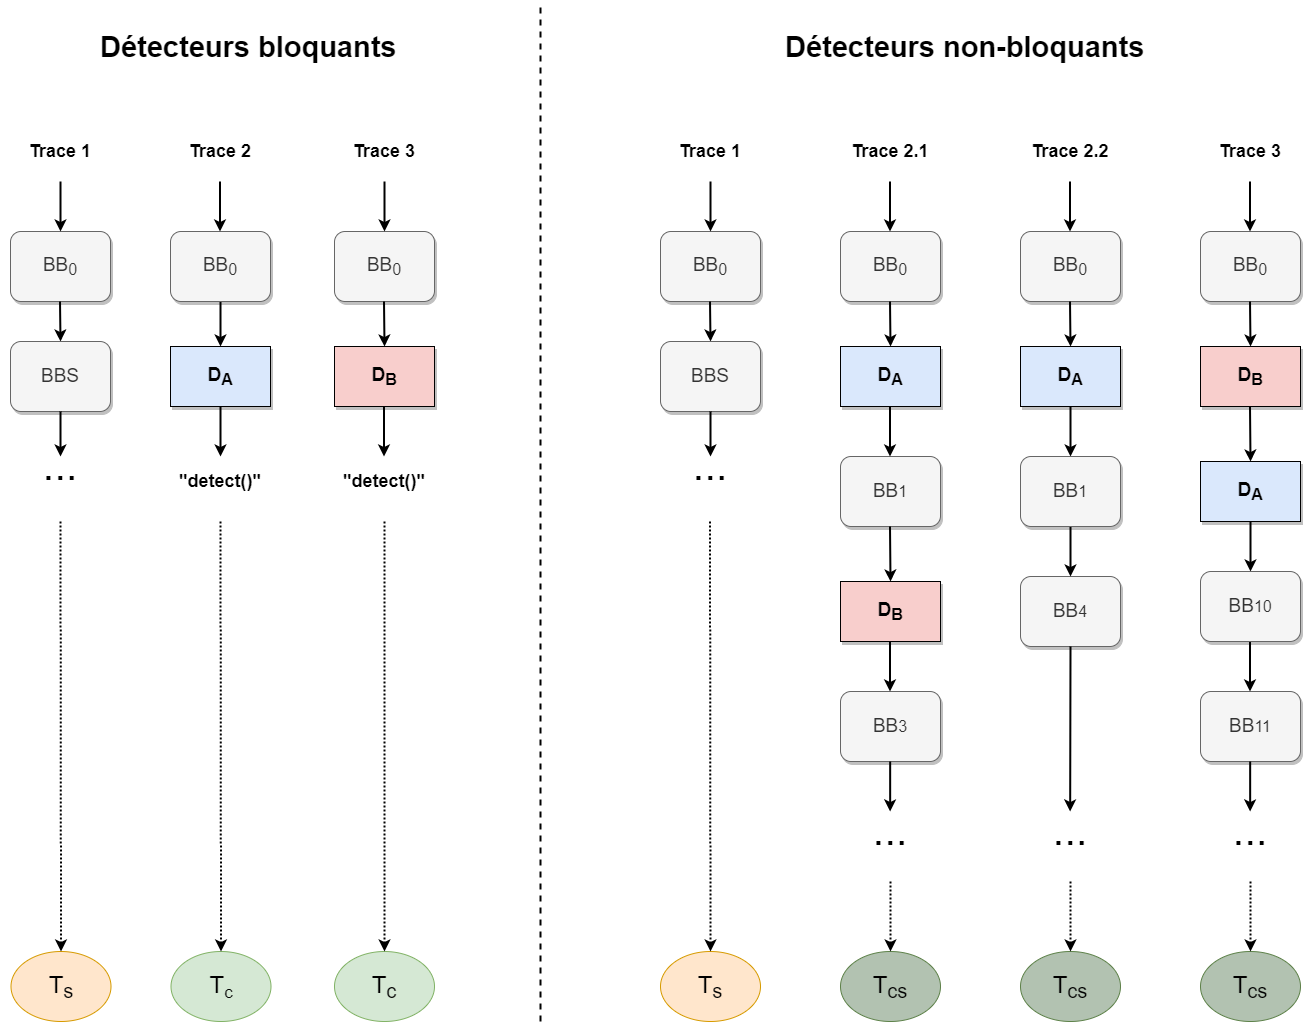
\includegraphics[scale=0.3]{ch6-ccpo/img/CCP-prop-stopping2.png}
                \caption{Exemples de traces avec détecteurs bloquants (à gauche) et non bloquants (à droite)}
                \label{fig:stop-not-to-stop}
            \end{figure}
            
        \subsection{Problématique de la couverture de $T_{cs}^{nb}(P, M)$} 
        \label{sec:ch6:valid-problematic}
        
            Dans la figure \ref{fig:stop-not-to-stop} précédente, on constate que si le détecteur $D_B$ est retiré (trace 3), alors toutes les traces d'exécution non bloquantes sont couvertes (définition \ref{def:valid}) par le détecteur $D_A$ (à l'exception de la trace 1 qui n'est de toute façon bloquée par aucun détecteur). En revanche, si on retire le détecteur $D_A$, alors il existe un chemin supplémentaire (trace 2.2) qui ne sera pas bloqué, le programme $P_{D_B}$ introduit donc au moins une nouvelle attaque par rapport aux programmes $P_{D_A, D_B}$ et $P_{D_A}$. L'ensemble de détecteurs optimal sera donc dans cet exemple $\{ D_A \}$. 
   
            \begin{defi} 
                \label{def:valid}
                Soit $Det(t)$ l'ensemble des détecteurs déclenchés dans une trace d'exécution $t$.
                Un ensemble de détecteurs $\mathcal{D}_i$ couvre un ensemble de traces $\mathcal{T}$ si chaque trace de $\mathcal{T}$ contient le déclenchement d'au moins un détecteur de $\mathcal{D}_i$:  
            \begin{equation*}
                Couvre(\mathcal{D}_i, \mathcal{T}) \equiv  t \in \mathcal{T} \mid \exists d \in \mathcal{D}_i  \mid  d \in Det(t)
            \end{equation*}                 
            \end{defi} 
            
            L'objectif étant de ne pas introduire de chemins d'attaques réussies, on s'intéresse aux attaques réussies et détectées (noté $T_{cs}(P, M)$).   
            Dans le cadre d'une exécution non bloquante, une attaque détectée termine en contre-mesure. 
            La notion d'attaque réussie pour des traces non bloquantes a du sens puisqu'on s'autorise à continuer après le déclenchement d'un détecteur afin de vérifier si l'objectif d'attaque aurait été validé dans le cas où les détecteurs ne seraient pas présents.                            
            Ainsi, les ensembles de détecteurs qui n'introduisent pas de nouvelles attaques sont ceux qui couvrent l'ensemble des traces d'attaques \textit{détectées et réussies} d'une exécution non bloquante (noté $T_{cs}^{nb}(P, M)$).
            La problématique \ref{probl:detector-optimization} revient donc à répondre à la problématique \ref{probl:detector-selection}, qui est un problème d'optimisation\footnote{La recherche de ces ensembles de détecteurs qui couvrent un ensemble de trace se rapproche de l'algorithme \textit{bloc-opt} évoqué dans le chapitre \ref{chpt:placement}.}.   

            \begin{probl}
                \label{probl:detector-selection}
                Trouver les ensembles $\mathcal{D}_i$ de détecteurs minimaux tels que chaque trace d'attaques détectées et réussies $T^{nb}_{cs}(P, M)$, pour un programme $P$ et un modèle d'attaquant $M$, soit couverte par au moins un détecteur de $\mathcal{D}_i$.
                Les ensembles minimaux sont ceux qui minimisent la fonction $\mathcal{W}(\mathcal{D})$ choisie par l'utilisateur.
            \end{probl}

            Pour la suite de cette section \ref{sec:ch6:ccpo}, on posera $\mathcal{T} = T^{nb}_{cs}(P, M)$.
            La recherche des ensembles $\mathcal{D}_i$ minimaux qui couvrent l'ensemble de trace $\mathcal{T}$ est réalisée en deux étapes:
            \begin{itemize}
                \item L'étape de classification (section \ref{sec:ch6:classification}) effectue une première passe sur les traces d'entrées afin de réduire l'espace de recherche.
                \item L'étape de sélection (section \ref{sec:ch6:selection}) consiste en la recherche des ensembles $\mathcal{D}_i$ optimaux  sur cet espace réduit.
            \end{itemize}
         
        \subsection{Classification des détecteurs}    
        \label{sec:ch6:classification}

            L'étape de classification consiste à faire un premier tri des traces d'entrées dans $\mathcal{T}$ pour trouver les détecteurs qui sont:
            \begin{itemize}
                \item \textit{inactifs}: ne se déclenchent jamais dans $\mathcal{T}$ et peuvent donc être écartés des ensembles minimaux.
                \item \textit{nécessaires}: se déclenchent au moins une fois seuls dans une trace d'exécution de $\mathcal{T}$ (sans qu'un autre détecteur ne soit déclenché), et doivent donc être conservés pour ne pas introduire de nouvelles attaques.
            \end{itemize}
            
            Tous les autres détecteurs sont dit \textit{répétitifs} et c'est sur ceux-ci qu'il faut effectuer la recherche d'ensembles minimaux.
            L'étape de \textit{classification} réduit l'espace d'exploration de la sélection des ensembles minimaux.
            En effet, seuls les détecteurs \textit{répétitifs} $\mathcal{D}_R$ doivent être considérés et seules les traces contenant uniquement des détecteurs répétitifs $\mathcal{T}_R$ (définition \ref{eq:tr}) doivent être couvertes (les traces contenant au moins un détecteur nécessaire seront de toute façon couvertes). 

            \begin{defi}[Ensemble des traces contenant uniquement des répétitifs]
                \label{eq:tr}
                \begin{equation*}
                    \mathcal{T}_{R} \equiv \forall t \in \mathcal{T} \mid Det(t) \cup \mathcal{D}_R
                \end{equation*}  
            \end{defi}
            
            La table \ref{tbl:vp-td-ccpa-classification} présente la classification des détecteurs du programme $vp2c+TD$ pour une limite de fautes jusqu'à 4\footnote{Cet exemple n'est pas étudié avec des entrées symboliques mais avec des tableaux d'entrées fixés.}. Les détecteurs peuvent être nécessaires ({\color{green!50} N}), répétitifs ({\color{orange!80} R}) ou inactifs ({\color{red!80} I}).
            
            \begin{table}[H]
            \centering
                \begin{tabular}{|l|c|c|c|c|c|c|c|c|c|c|c|}
                \hline
                \rowcolor[HTML]{EFEFEF} 
                Détecteur & $D_0$ & $D_1$ & $D_2$ & $D_3$ & $D_4$ & $D_5$ & $D_6$ & $D_7$ & $D_8$ & $D_9$ & $D_{10}$ \\ \hline
                \rowcolor[HTML]{FFCCC9} 
                \cellcolor[HTML]{EFEFEF}1 faute & I & I & I & \cellcolor[HTML]{FFCC67}R & I & I & I & I & \cellcolor[HTML]{9AFF99}N & I & \cellcolor[HTML]{FFCC67}R \\ \hline
                \rowcolor[HTML]{FFCC67} 
                \cellcolor[HTML]{EFEFEF}2 fautes & R & \cellcolor[HTML]{FFCCC9}I & R & R & R & R & R & R & \cellcolor[HTML]{9AFF99}N & \cellcolor[HTML]{FFCCC9}I & \cellcolor[HTML]{9AFF99}N \\ \hline
                \rowcolor[HTML]{9AFF99} 
                \cellcolor[HTML]{EFEFEF}3 fautes & N & \cellcolor[HTML]{FFCCC9}I & N & N & N & N & \cellcolor[HTML]{FFCC67}R & N & N & \cellcolor[HTML]{FFCCC9}I & N \\ \hline
                \rowcolor[HTML]{9AFF99} 
                \cellcolor[HTML]{EFEFEF}4 fautes & N & \cellcolor[HTML]{FFCCC9}I & N & N & N & N & \cellcolor[HTML]{FFCC67}R & N & N & \cellcolor[HTML]{FFCCC9}I & N \\ \hline
                \end{tabular}
            \caption{Classification des détecteurs pour $vp2c+TD$ en fonction du nombre d'inversion de test maximum}
            \label{tbl:vp-td-ccpa-classification}
            \end{table}
                
            Les détecteurs $D_1$ et $D_9$ sont inactifs quel que soit le nombre de fautes, ce qui s'explique par le fait qu'ils protègent des branches qui n'ont pas d'impact sur l'objectif d'attaque (respectivement ligne 12 et 18 de la fonction \texttt{verify\_pin} du listing \ref{lst:ch6:vp4-vp}). A l'inverse, le détecteur $D_8$ est nécessaire même en faute unique, étant donné que l'inversion de l'appel à la fonction \texttt{compare} permet de gagner en une faute.
            
        \subsection{Sélection des détecteurs}
        \label{sec:ch6:selection} 

            La seconde étape de la méthodologie consiste à chercher les ensembles de détecteurs répétitifs $\mathcal{D}_{Ri}$ qui, associés aux détecteurs nécessaires $\mathcal{D}_N$, couvrent l'ensemble des traces de $\mathcal{T}_R$. 
            La recherche des $\mathcal{D}_{Ri}$ optimaux est ainsi un problème d'optimisation, dont l'implémentation sera précisée dans la section \ref{sec:ccpo-impl}.

            Dans le cas de l'exemple $vp2+TD$ en deux fautes, seules deux traces d'attaques détectées réussies contiennent uniquement des détecteurs répétitifs, notées $a_1$ et $a_2$.
            Les figures \ref{tbl:trace-o1.19} et \ref{tbl:trace-o2.32} présentent respectivement l'attaque $a_1$ en une faute et l'attaque $a_2$ en deux fautes, sans prendre en compte les transitions qui ne sont pas des fautes ou des détections.
            Deux ensembles de détecteurs répétitifs $\{ D_3 \}$ et $\{ D_7 \}$ permettent de couvrir $\mathcal{T}_R = \{ a_1, a_2 \}$, et doivent être associés aux détecteurs nécessaires $\mathcal{D}_N = \{D_{8}, D_{10}\}$ pour couvrir $\mathcal{T}$:
            \begin{itemize}
                \item $\mathcal{D}_1 = \{D_3, D_8, D_{10}\}$
                \item $\mathcal{D}_2 = \{D_7, D_8, D_{10}\}$
            \end{itemize}
             
            \begin{table}[ht]
            \centering                
                \begin{tabular}{|
                >{\columncolor[HTML]{C0C0C0}}c |
                >{\columncolor[HTML]{ECF4FF}}c |
                >{\columncolor[HTML]{ECF4FF}}l |
                >{\columncolor[HTML]{FFCCC9}}c |
                >{\columncolor[HTML]{ECF4FF}}l |
                >{\columncolor[HTML]{CBCEFB}}c |
                >{\columncolor[HTML]{ECF4FF}}c |
                >{\columncolor[HTML]{CBCEFB}}c |
                >{\columncolor[HTML]{ECF4FF}}c |}
                \hline
                Trace $a_1$ & \multicolumn{2}{c|}{\cellcolor[HTML]{ECF4FF}...} & Faute (bb2) & ... & Dét 3 & ... & Dét 7 & ... \\ \hline
                \end{tabular}
            \caption{Trace de l'attaque réussie détectée $a_1$ \label{tbl:trace-o1.19}}
            \end{table}
                                
            \begin{table}[ht]
            \centering
                \begin{tabular}{|
                >{\columncolor[HTML]{C0C0C0}}c |
                >{\columncolor[HTML]{ECF4FF}}c |
                >{\columncolor[HTML]{ECF4FF}}l |
                >{\columncolor[HTML]{FFCCC9}}c |
                >{\columncolor[HTML]{ECF4FF}}l |
                >{\columncolor[HTML]{CBCEFB}}c |
                >{\columncolor[HTML]{ECF4FF}}c |
                >{\columncolor[HTML]{FFCCC9}}l |
                >{\columncolor[HTML]{ECF4FF}}c |
                >{\columncolor[HTML]{CBCEFB}}c |
                >{\columncolor[HTML]{ECF4FF}}c |}
                \hline
                Trace $a_2$ & \multicolumn{2}{c|}{\cellcolor[HTML]{ECF4FF}...} & Faute (bb2) & ... & Dét 3 & ... & Faute (bb3) & ... & Dét 7 & ... \\ \hline
                \end{tabular}
            \caption{Trace de l'attaque réussie détectée $a_2$ \label{tbl:trace-o2.32}}
            \end{table}
        
            En fonction de la pondération $\mathcal{W}$ choisie, $\mathcal{D}_{1}$ ou $\mathcal{D}_{2}$ seront sélectionnés. 
            Pour une pondération égale pour chaque détecteur, $\mathcal{D}_{1}$ et $\mathcal{D}_{2}$ sont équivalents, mais le détecteur $D_3$ correspond à la duplication de la branche fausse du test \texttt{i < size} dans la boucle et pourrait par conséquent être considéré comme plus coûteux que le détecteur $D_7$ (duplication de $D_{10}$, hors de la boucle), privilégiant ainsi l'ensemble $\mathcal{D}_{2}$.  
            Les listing \ref{lst:ch6:vp4-vp-res} et \ref{lst:ch6:vp4-compare-res} présentent les parties du code retirées (en {\color{Red}rouge}) et conservées (en {\color{OliveGreen}vert}) pour l'ensemble $\mathcal{D}_{1}$, pour respectivement les fonctions \texttt{verify\_pin} et \texttt{compare}. Le corps de contre-mesure (ici chaque variable locale $c_i$ associée à des détecteurs retirés) est également retiré.

        \subsection{Conclusion}
        \label{sec:ch6:pres-conclusion} 
                 
            La méthodologie de calcul de l'ensemble de détecteurs minimaux est ainsi découpée en deux étapes, la \textit{classification} et la \textit{sélection}, comme le montre la figure \ref{fig:ccpo-scheme}.            
            Ainsi, une seule exploration des exécutions est effectuée sur le programme $P$ contenant tous les détecteurs. Cette méthodologie impose cependant que l'évaluation de la condition d'un détecteur n'ait pas d'effet de bord sur l'exécution de la suite du programme ainsi que sur l'objectif d'attaque étudié. 
            La correction de cette approche, correspondant à la garantie qu'aucune nouvelle attaque n'est introduite par le retrait des détecteurs, est discutée en section \ref{sec:ccpo-formalisation}.
               
            \begin{figure}[!ht]\centering
                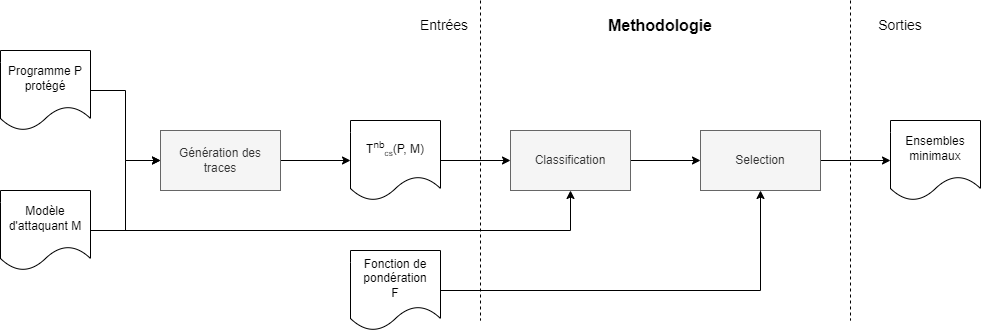
\includegraphics[scale=0.4]{ch6-ccpo/img/ccpo-scheme-select.drawio.png}
                \caption{Schéma de la méthodologie d'optimisation de détecteurs}
                \label{fig:ccpo-scheme}
            \end{figure}
    
            La problématique de l'optimisation des contre-mesures a été abordée dans les chapitres précédents et la méthodologie présentée dans ce chapitre propose une solution dans le cas des contre-mesures à détecteurs, visant à répondre à la problématique \ref{probl:detector-optimization}.
            L'optimisation de détecteurs est une forme de comparaison de programmes protégés puisqu'il s'agit de comparer les différentes variations $\mathcal{V}(P)$.            
            Elle peut aussi être utilisée en amont du processus de développement lors de l'application des contres-mesures pour aider au placement de ces contre-mesures.        
    
            La méthodologie présentée ici garantit que les détecteurs peuvent être retirés sans introduire de nouvelles attaques. Néanmoins, déterminer quelles portions du \textit{corps de contre-mesure} peuvent être enlevées par rapport à l'ensemble de détecteurs calculé n'est pas trivial dans le cas général.
            La figure \ref{fig:ccpo-metho} présente les différents cas d'utilisation de la méthodologie en fonction de la méthode de placement utilisée pour le programme $P$ : placement automatique (a) ou placement manuel (b).
            Le scénario (a) correspond au cas où le placement est effectué à l'aide d'un outil automatique, que ce soit par un outil dédié \cite{lalande} ou un compilateur \cite{Reis/ISCCO05, Proy/TACO17}.
            Il s'agit ici du scénario de l'exemple $vp2c+TD$ où la duplication de test peut être appliquée avec une granularité de l'ordre du point d'injection. 
            Dans ce cas, le programme protégé $P'$ est simplement régénéré à partir d'un ensemble de détecteurs calculé par l'algorithme d'optimisation : 
            \begin{enumerate}
                \item Appliquer systématiquement les contre-mesures.
                \item Calculer un ensemble optimal de détecteurs $D_i$.
                \item Appliquer le placement avec les détecteurs de $D_i$ uniquement.
            \end{enumerate}
    
            \begin{figure}[!ht]
            \centering
                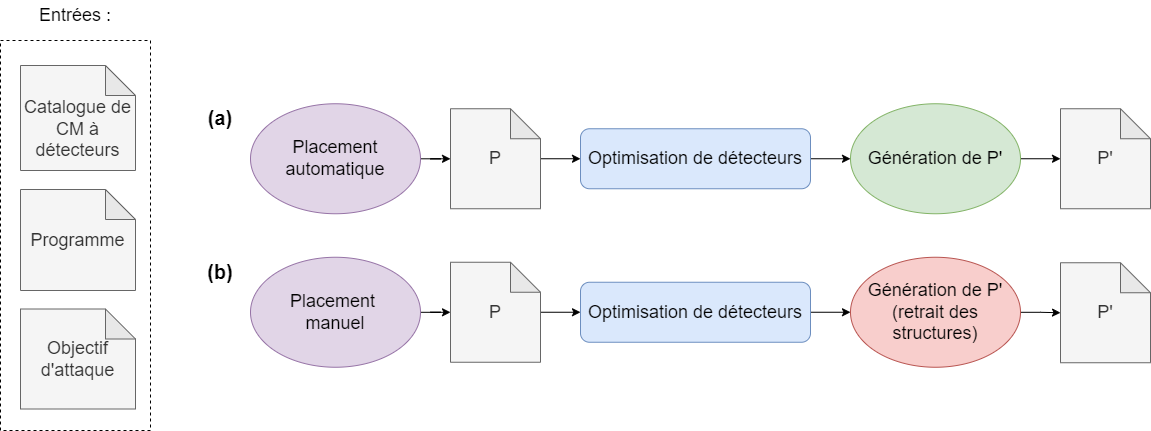
\includegraphics[scale=0.33]{ch6-ccpo/img/placement-ccpo2.drawio.png}
                \caption{Différentes applications de la méthodologie}
                \label{fig:ccpo-metho}
            \end{figure}
    
            Le scénario (b) décrit le cas où il n'est pas possible de ré-appliquer automatiquement la contre-mesure à l'aide de l'ensemble $D_i$. Cela implique qu'il faut calculer le corps de contre-mesure pouvant être retiré.
            Cette analyse n'est pas triviale puisqu'elle requiert de prendre en compte toutes les fautes possibles de manière à déterminer si une portion du corps de contre-mesure est nécessaire.
            Cette partie de la problématique n'est pas traitée dans ce manuscrit.
    
            Un dernier cas d'utilisation peut être noté et correspond à un cas particulier du scénario a, où le placement automatique est un placement \textit{optimal} (comme décrit dans le chapitre précédent). Dans ce cas, la méthodologie peut être utilisée pour vérifier l'optimalité du placement, celui-ci dépendant de la complétude et correction de l'exploration des chemins d'attaques fautés\footnote{De la même manière, l'optimisation de détecteurs repose sur la complétude et la correction des chemins d'attaques détectées.}.
      
    \section{Garanties de la méthode et protection des détecteurs}
    \label{sec:ccpo-formalisation}

        Cette section s'intéresse aux garanties de la méthodologie présentée dans la section précédente, en supposant l'exploration des chemins $T^{nb}_{cs}(P, M)$ complète et correcte.
        La section \ref{sec:exec-classification} revient sur les différentes classes d'exécution dans le cadre d'une exécution avec détecteurs non bloquants et la section \ref{sec:ccpo-rob-preserv} indique les relations autorisées entre ces classes pour préserver la robustesse du programme $P'$.
        La section \ref{sec:ccpo-trace-match} explique comment les traces d'attaques peuvent être mises en correspondance avec les traces d'attaques des différentes variations du programme $P$, permettant ainsi de vérifier que les attaques détectées dans $P$ resteront détectées dans le programme $P'$.
        Enfin, la section \ref{sec:ccpo-prot-det} s'intéresse aux possibles faux positifs et présente une solution appelée \og protection des détecteurs \fg{}. 
        
        \subsection{Classification des exécutions pour $T^{nb}(P, M)$}
        \label{sec:exec-classification}
    
            Les exécutions d'un programme peuvent être caractérisées par:
            \begin{itemize}
                \item la validation ou non de l'objectif d'attaque $\phi$.
                \item la terminaison (exécution terminée ou timeout/boucle infinie).
                \item la présence ou non de fautes.
                \item le déclenchement d'une contre-mesure (d'un détecteur).
            \end{itemize}
            
            Si on choisit d'abstraire la terminaison dans l'objectif d'attaque, ainsi que les cas d'erreurs (crash, division par zéro, accès mémoire invalide), cela permet de simplifier les catégories de traces en laissant l'utilisateur définir, dans l'objectif d'attaque, s'il considère un timeout ou une double désallocation avec \texttt{free} par exemple, comme une attaque réussie.
            C'est ce qui est fait dans Lazart, dans lequel l'utilisateur peut paramétrer les types de terminaison correspondant à une attaque réussie (voir section \ref{sec:lazart-aa}).
            
            Classiquement, les exécutions ou les traces d'exécutions, pour un programme $P$ et un modèle de faute $M$, sont partitionnées dans les ensembles suivants :
            \begin{itemize}
                \item $T_n(P, M)$: les exécutions nominales (sans fautes).
                \item $T_c(P, M)$: les attaques terminant en contre-mesure (détectées).
                \item $T_s(P, M)$: les attaques réussies ($\phi$ satisfait) et non détectées.
                \item $T_f(P, M)$: les attaques non réussies ($\phi$ non satisfait) et non détectées.
            \end{itemize}
            
            Dans le cas d'une analyse avec détecteurs non bloquants, l'exécution ne peut plus terminer en contre-mesure. 
            Pour autant il est possible de différencier les traces contenant le déclenchement d'un détecteur et celles n'en contenant pas.
            De plus, il est possible d'évaluer la condition de succès de l'objectif d'attaque, l'exécution n'étant plus interrompue par les détecteurs.
            Pour une exécution non bloquante, les traces produites à partir de $T_c(P, M)$ peuvent se décomposer en:
            \begin{itemize}
                \item $T_{cs}(P, M)$: les attaques dans lesquelles au moins un détecteur a été déclenché et où l'objectif d'attaque $\phi$ est validé.
                \item $T_{cf}(P, M)$: les attaques dans lesquelles au moins un détecteur a été déclenché et où $\phi$ n'est pas satisfait.
            \end{itemize}
       
            \begin{table}[h]
            \centering
                \begin{tabular}{|l|l|l|l|l}
                \cline{1-4}
                Ensemble / Caractéristique & $\phi$ & fautes & détecteurs                                                                                                                                                                               &  \\ \cline{1-4}
                $T_n(P, M)$                   & faux\footnotemark    & 0      & 0\footnotemark &  \\ \cline{1-4}
                $T_s(P, M)$                   & vrai   & 1+     & 0                                                                                                                                                                                        &  \\ \cline{1-4}
                $T_{cs}(P, M)$                & vrai   & 1+     & 1+                                                                                                                                                                                       &  \\ \cline{1-4}
                $T_{cf}(P, M)$                & faux   & 1+     & 1+                                                                                                                                                                                       &  \\ \cline{1-4}
                $T_f(P, M)$                   & faux   & 1+     & 0                                                                                                                                                                                        &  \\ \cline{1-4}
                \end{tabular}
            \caption{Caractéristiques des différents ensembles de traces d'exécution\label{tbl:traces-categories}}
            \end{table}

            \footnotetext[7]{On suppose que l'objectif d'attaque ne peut pas être validé dans une exécution nominale.}
            \footnotetext[8]{On suppose que les détecteurs ne se déclenchent pas dans une exécution nominale, la contre-mesure préservant le comportement observable du programme en l'absence de faute.}

            La table \ref{tbl:traces-categories} présente les caractéristiques (nombre de fautes, validation de l'objectif d'attaque et nombre de déclencheurs déclenchés) pour les cinq classes de traces d'exécution, ces ensembles de traces étant disjoints.
            
        \subsection{Préservation de la robustesse}
        \label{sec:ccpo-rob-preserv}

            Le paradoxe de dilution \cite{Dureuil/Phd16}, énoncé dans le chapitre précédent, explique qu'il soit difficile de comparer les attaques de différentes versions protégées d'un programme. Les contre-mesures ajoutent des chemins d'exécution et de la surface d'attaque.
            S'il est possible d'associer chaque trace d'exécution d'un programme $P$ à des traces d'un programme $P'$ à l'aide d'une fonction $\delta$, alors pour que $P'$ soit au moins aussi robuste que $P$, il faut que chacune des traces qui ne sont pas des attaques réussies pour $P$ restent inefficaces (attaques bloquées ou objectif d'attaque non réussi) pour $P'$. La table \ref{tbl:trace-class-changes-nb} présente les classes autorisées pour les traces de $T(P')$ en fonction des traces correspondantes (par une fonction $\delta$) dans $T(P)$ pour une conservation de la robustesse.
                                
            \begin{table}[h]
            \centering
                \begin{tabular}{|l|ccccc|}
                \hline
                \multicolumn{1}{|c|}{\multirow{2}{*}{Classe de $t \in T(P)$}} & \multicolumn{5}{c|}{Classes autorisées pour $t' \in \delta(t)$}                                                                                                                              \\ \cline{2-6} 
                \multicolumn{1}{|c|}{}                                        & \multicolumn{1}{l|}{$T_n(P', M)$} & \multicolumn{1}{l|}{$T_s(P', M)$} & \multicolumn{1}{l|}{$T_{cs}(P', M)$} & \multicolumn{1}{l|}{$T_{cf}(P', M)$} & \multicolumn{1}{l|}{$T_f(P', M)$} \\ \hline
                $T_n(P, M)$                                                   & \multicolumn{1}{c|}{\checkmark}   & \multicolumn{1}{c|}{\xmark}       & \multicolumn{1}{c|}{\checkmark}      & \multicolumn{1}{c|}{\checkmark}      & \checkmark                        \\ \hline
                $T_s(P, M)$                                                   & \multicolumn{1}{c|}{\checkmark}   & \multicolumn{1}{c|}{\checkmark}   & \multicolumn{1}{c|}{\checkmark}      & \multicolumn{1}{c|}{\checkmark}      & \checkmark                        \\ \hline
                $T_{cs}(P, M)$                                                & \multicolumn{1}{c|}{\checkmark}   & \multicolumn{1}{c|}{\xmark}       & \multicolumn{1}{c|}{\checkmark}      & \multicolumn{1}{c|}{\checkmark}      & \checkmark                        \\ \hline
                $T_{cf}(P, M)$                                                & \multicolumn{1}{c|}{\checkmark}   & \multicolumn{1}{c|}{\xmark}       & \multicolumn{1}{c|}{\checkmark}      & \multicolumn{1}{c|}{\checkmark}      & \checkmark                        \\ \hline
                $T_f(P, M)$                                                   & \multicolumn{1}{c|}{\checkmark}   & \multicolumn{1}{c|}{\xmark}       & \multicolumn{1}{c|}{\checkmark}      & \multicolumn{1}{c|}{\checkmark}      & \checkmark                        \\ \hline
                \end{tabular}
            \caption{Classes autorisées pour les traces $t' \in f(t)$ \label{tbl:trace-class-changes-nb}}
            \end{table}
            
            L'optimisation de détecteurs implique qu'un programme $P'$ puisse avoir des attaques réussies (non détectées) nécessitant moins de fautes que leur attaque correspondante dans $P$, c'est-à-dire $|F(t')| < |F(t)|, t \in T_s(P, M), t' \in T_s(P', M), t' \in \delta(t)$ (avec $F(t)$ la liste ordonnée des fautes dans la trace $t$). 

        \subsection{Correspondances entre les traces}          
        \label{sec:ccpo-trace-match}
            
            \begin{figure}[htbp]
            \centering
                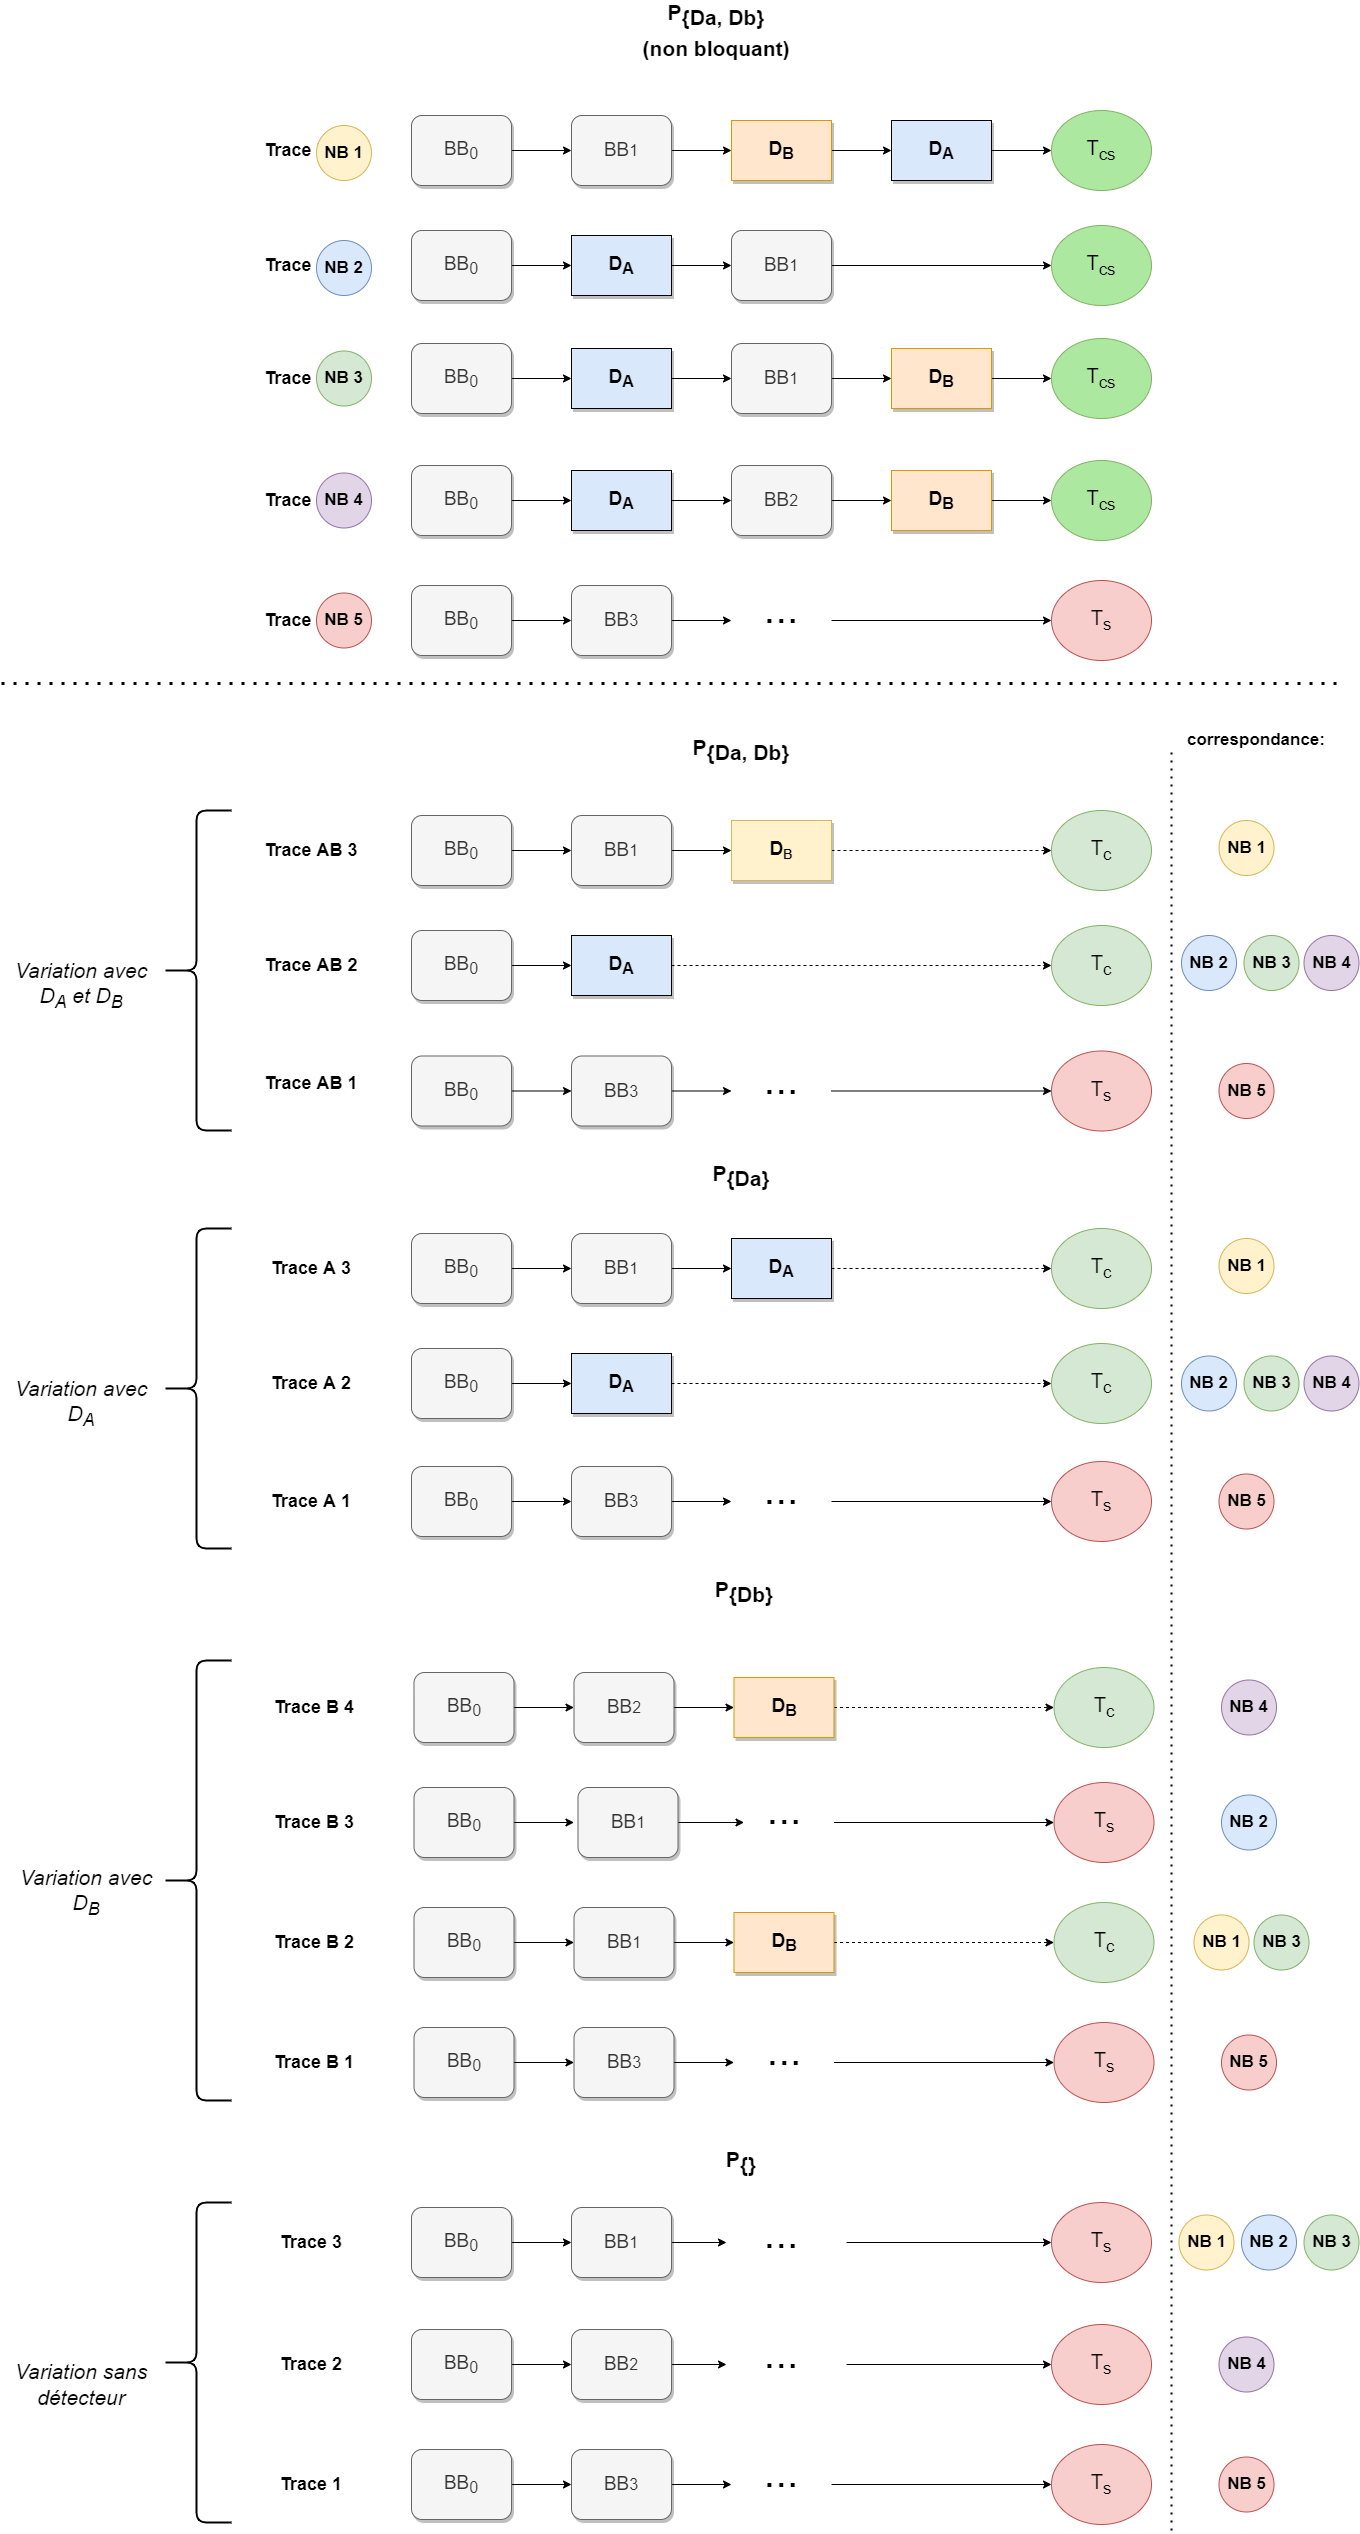
\includegraphics[scale=0.27]{ch6-ccpo/img/trace-corresp.drawio.png}
            \caption{Exemple de correspondance entre les traces des différentes variations $\mathcal{V}(P)$}
            \label{fig:ch6:trace-corresp}
            \end{figure}

            Cette section vise à établir les correspondances entre les traces d'attaques des différentes variations de $P$ et les traces d'exécution avec détecteurs non bloquants sur le programme $P$.     
            Une trace d'exécution bloquante peut correspondre à plusieurs traces d'exécutions non bloquantes. Dans ce cas, la trace bloquante (définition \ref{def:block-trace}) est un préfixe de chaque trace non bloquante correspondante (définition \ref{def:nonblock-trace}).
            
            \begin{defi}
                \label{def:block-trace}
                Les traces d'attaque détectée avec détecteurs bloquants $T_c(P, M)$ sont de la forme $s_0 ... s_n d_i$, avec $s_i$ les transitions nominales ou fautées et $d_i$ le déclenchement d'un détecteur.
            \end{defi}
            
            \begin{defi}
                \label{def:nonblock-trace}
                Les traces d'attaque détectée avec détecteurs non bloquants $T_{c}^{nb}(P, M)$ sont de la forme $s^1_0 ... s^1_{n_1} d_i s^2_0 ... s^2_{n_2} d_j ...$ avec $s^i_j$ les transitions nominales ou fautées et $d_i$ les déclenchements de détecteurs.
            \end{defi}
                    
            La figure \ref{fig:ch6:trace-corresp} présente les correspondances entre les traces des différentes variations d'un programme $P$ contenant deux détecteurs $D_A$ et $D_B$, et les traces de l'exécution non bloquante $T^{nb}(P)$ (en haut).
            Pour chaque trace d'exécution, sa classe peut être attaque réussie ($T_s$) ou attaque détectée ($T_c$). 
            Dans le cas de l'exécution non bloquante, les traces d'attaques réussies et détectées sont indiquées par $T_{cs}$.
            Dans cet exemple, les ensembles de détecteurs $\{D_B\}$ et $\{\}$ ne permettent pas de couvrir l'ensemble des attaques de $T^{nb}$ et les programmes $P_{D_B}$ et $P_{\{\}}$ introduisent de nouvelles attaques réussies qui ne sont pas détectées (respectivement les traces $B3$ et les traces $2$ et $3$).
            
            L'exploration des exécutions non bloquantes du programme $P$ contenant tous les détecteurs permet ainsi d'évaluer la robustesse de chaque variation de $P$.
            Si toutes les traces de $T^{nb}_{cs}{P}$ sont couvertes par (au moins) un détecteur d'un ensemble $\mathcal{D}_{i}$, alors les traces correspondante dans $P_{\mathcal{D}_{i}}$ seront détectées (dans $T_c(P_{\mathcal{D}_{i}})$).
            Cela implique cependant que les conditions des détecteurs non bloquants n'aient pas d'effet de bord sur le reste de l'exécution du programme (et l'objectif d'attaque).
                     
        \subsection{Protection des détecteurs}
        \label{sec:ccpo-prot-det}

            L'analyse de l'ensemble $T^{nb}_{cs}(P, M)$ peut néanmoins générer des faux positifs, puisqu'il existe certaines exécutions qui peuvent fausser l'analyse, en classifiant un détecteur comme \textit{nécessaire} de manière incorrecte. Il s'agit des fautes qui forcent le déclenchement d'un détecteur (alors que la condition de détection est fausse).
             
            Le problème s'illustre facilement avec le modèle d'inversion de test, où la notion de \textit{forcer le passage dans un détecteur} est plus claire.
            L'extrait de programme \ref{lst:detector-base} contient un simple détecteur avec pour condition \texttt{c}. Si l'exploration des exécutions fautées est complète, et qu'il existe des exécutions où $c$ est faux avec encore (au moins) une faute de disponible, alors il existe un ensemble d'exécutions dans lesquelles le test est inversé pour forcer l'entrée dans le détecteur.
                
\begin{minipage}{0.93\linewidth}
\lstset{escapeinside={<@}{@>}}
\lstset{caption={Exemple de trace forcant le passage en contre-mesure},label=lst:detector-base, numbers=left,xleftmargin=2em}
\begin{lstlisting}
...

if(c) {
countermeasure("X");
}

...\end{lstlisting} 
\end{minipage}

            L'ensemble de ces traces donnant lieu à une sur-approximation de la méthodologie est nommé $T^{nb}_{b}(P, M)$ et est contenu dans $T_{cs}(P, M)$. La recherche des ensembles minimaux de détecteurs doit donc s'effectuer sur $T^{nb}_{cs}(P, M) / T^{nb}_{b}(P, M)$.
            Trouver les traces $T^{nb}_b(P, M)$ à partir de $T^{nb}_{cs}(P, M)$ n'est pas trivial, mais une solution consiste à interdire les fautes forçant le passage vers la branche \textit{vraie} des détecteurs au niveau de la génération des traces. C'est cette approche qui est implémentée dans Lazart.
                
    \section{Implémentation et expérimentations}
    \label{sec:ccpo-impl}

        Cette section présente les résultats obtenus pour la méthodologie décrite dans ce chapitre et son implémentation au sein de l'outil Lazart.
        
        \subsection{Implémentation dans Lazart}
        \label{sec:ch6-impl}

            Cette section présente l'implémentation de la méthodologie d'optimisation de détecteurs au sein de Lazart.
            La section \ref{sec:ch6-non block} revient sur l'implémentation des détecteurs non bloquants. 
            Les sections \ref{sec:ch6-impl-classification} et \ref{sec:ch6-impl-selection} détaillent respectivement les étapes de classification et de sélection.
            Enfin, la section \ref{sec:ch6-supdect} discute de la problématique de la création de \textit{super-détecteur} lors de l'application automatique de certaines contre-mesures.

            \subsubsection{Détecteurs non bloquants}
            \label{sec:ch6-non block}
        
                Usuellement, les outils d'analyses considèrent la terminaison d'une exécution en contre-mesure comme un type de terminaison à part entière.                 
                Pour l'analyse de contre-mesures présentée dans ce chapitre, il est nécessaire de supporter un mode d'exécution dans lequel les détecteurs ne terminent pas l'exécution du programme, tout en gardant en mémoire les détecteurs déclenchés. 
                Le déclenchement d'un détecteur $D_i$ est traduit par un évènement de type spécifique qui est affiché sur la sortie pour être récupérée lors du rejeu (voir section \ref{sec:lazart-impl-klee-replay}).   
            
                En pratique, la fonction associée au déclenchement d'un détecteur bloquant correspond au code C présenté dans le listing \ref{lst:trigger-fct-stop}. Le paramètre \texttt{\_det\_id} correspond à l'identifiant unique du détecteur déclenché, en tant que chaîne de caractères. 
                L'exécution est arrêtée avec un appel à \texttt{klee\_assume(false);}.
    
\lstset{style=codeC, caption={Fonction de déclenchement de détecteur bloquant},label={lst:trigger-fct-stop}}
\begin{lstlisting}     
void _LZ__trigger_detector_stop(const char* _det_id)
{
    _LZ__detector_alarm_ = true;
    if(klee_is_replay())
        printf("\n[CM] triggered %s \n", _det_id);  // See wiki for print syntax.
    klee_assume(false); // Cut exploration.
}
\end{lstlisting}  

                \begin{sloppypar}
                Le listing \ref{lst:trigger-fct-nb} correspond à la fonction pour un détecteur non bloquant, qui ne diffère que par l'absence de l'appel à \texttt{klee\_assume(false);}.
                La variable globale \texttt{\_LZ\_\_detector\_alarm\_} permet de vérifier dans l'objectif d'attaque si au moins un détecteur a été déclenché. 
                La question de savoir si une attaque est détectée peut également se faire en vérifiant si $Det(t) = \emptyset$ dans l'\gls{api} Python.
                \end{sloppypar}
    
\lstset{style=codeC, caption={Fonction de déclenchement d'un détecteur non bloquant},label=lst:trigger-fct-nb}
\begin{lstlisting}     
void _LZ__trigger_detector(const char* _det_id)
{
    _LZ__detector_alarm_ = true;    
    if(klee_is_replay()) 
        printf("\n[CM] triggered %s \n", _det_id); // See wiki for print syntax.
}

\end{lstlisting}  

                Dans le cas d'une exécution symbolique complète et correcte, une analyse d'attaque avec des détecteurs bloquants ou non bloquants n'a pas d'impact sur les chemins d'attaques réussies obtenus.
                En effet, seuls des chemins d'attaques détectées peuvent être générés à partir d'un détecteur non bloquant.
                Le mode bloquant a l'avantage d'arrêter plus tôt l'exploration des attaques détectées et donc de réduire le temps de l'exploration. C'est pourquoi il s'agit du mode par défaut pour les analyses d'attaques, les détecteurs non bloquants étant réservés à l'optimisation de détecteurs.
            
            \subsubsection{Classification}
            \label{sec:ch6-impl-classification}
    
                 La première étape de classification est effectuée sur l'ensemble des traces d'attaques réussies et détectées, dans une exécution non bloquante.
                 La classification des détecteurs repose sur le calcul du \textit{niveau de répétition minimal} $L_m[D_i]$ de chaque détecteur $D_i$ sur l'ensemble des traces.              
                 Pour chaque trace, on calcule le \textit{niveau de répétition} qui correspond au nombre de détecteurs \textit{différents} déclenchés dans cette trace (c'est-à-dire sans prendre en compte les répétition d'un même détecteur au sein de la trace).
                 $L_m[D_i]$ qui est initialisé à $\infty$ et est mis à jour à chaque trace pour chaque détecteur présent.
                 Chaque détecteur est finalement classé en fonction de ce niveau de répétition minimal :
                \begin{itemize}
                    \item Inactif: si $L_m[D_i] = \infty$ \textit{(ne s'est jamais déclenché)}
                    \item Nécessaire: si $L_m[D_i] = 1$
                    \item Répétitif: si $L_m[D_i] \in \; ]1; \infty[$
                \end{itemize}
    
                L'implémentation utilise une classification en deux étapes, permettant d'obtenir les résultats pour chaque nombre de fautes jusqu'à $n$ fautes.
                Dans un premier temps, la \textit{classification locale} est calculée, correspondant au calcul de la classe de chaque détecteur pour un nombre de fautes donné.
                Dans un second temps, la classification globale est calculée, en fonction de la classification locale pour les nombres de fautes inférieurs (correspondant à une relation d'ordre $inactif < repetitif < necessaire$:
                \begin{itemize}
                    \item si un détecteur est \textit{répétitif} en $n$ fautes, il est \textit{répétitif} ou \textit{nécessaire} en $m$ fautes pour $m \geq n$.
                    \item si un détecteur est \textit{nécessaire} en $n$ fautes, il est \textit{nécessaire} en $m$ fautes pour $m \geq n$.
                \end{itemize}
                
            \subsubsection{Étape de sélection}
            \label{sec:ch6-impl-selection}
    
               Pour rappel, l'étape de sélection vise à trouver les ensembles minimaux (selon la fonction de pondération $\mathcal{W}$) de détecteurs répétitifs (dans $\mathcal{D}_R$) qui couvrent l'ensemble des traces $\mathcal{T}_R$. 
               Une première solution consiste à essayer toutes les combinaisons de détecteurs possibles, et de conserver uniquement les ensembles qui couvrent $\mathcal{T}_R$.
               
               L'algorithme présenté dans le listing \ref{lst:ch6-select} présente le pseudo code de l'algorithme de sélection utilisé dans Lazart.
               Celui-ci vise à explorer les ensembles de détecteurs contenant un seul élément (ajoutés à la pile, lignes 4 à 6) et explorer progressivement les ensembles contenant un élément de plus.
               L'ensemble des solutions minimales (\texttt{bests}) est initialisé avec l'ensemble $\mathcal{D}_r$.
               L'objectif est d'arrêter l'exploration lorsqu'un ensemble est d'ores et déjà supérieur aux minimums courants\footnote{Par exemple: si $\{D_{1}\}$ couvre l'ensemble de traces, alors $\{D_{1}, D_2\}$ le couvre aussi. Cependant l'ensemble $\{D_{1}, D_2\}$ ne peut pas être une solution minimale puisqu'il a un poids plus élevé et il n'est pas nécessaire d'explorer les ensembles plus grands. En revanche, il est nécessaire d'explorer $\{D_{2}\}$ qui pourrait faire partie des solutions minimales.} (lignes 11 et 12).
               Si un ensemble ne couvre pas $\mathcal{T}_R$ et qu'il n'a pas un poids supérieur aux ensembles minimaux déjà trouvés, alors les ensembles avec un détecteur de plus sont ajoutés à la liste des ensembles à explorer (lignes 22 à 25).

\lstset{language=python, caption={Pseudo-code de l'algorithme de sélection},label=lst:ch6-select}
\begin{lstlisting}
def selection(traces, repetitives):
bests = [repetitives] # Current best sets covering traces.

set_stack = [] # Stack of set to be checked, by total weight (W)
for det in repetitives: 
set_stack += [det] # Initialize with singletons.

while set_stack not empty:
curr = set_stack.pop()

if W(curr) > W(bests[0]):  
    continue # Stop exploration for super-sets

if Cover(curr, traces): 
    # Update best sets.
    if W(curr) == W(bests[0]):
        bests += curr
    elif W(curr) < W(bests[0]):
        bests = [curr]
        
    continue # Stop exploration for super-sets
else: # Add super-sets to stack
    for det in repetitives:
        if det not in curr:
            set_stacks.insert(curr + [det])

return bests
\end{lstlisting} 
           
                La complexité de cet algorithme est dépendante du nombre de détecteurs répétitifs $\mathcal{D}_{R}$ ainsi que du nombre de traces dans $\mathcal{T}_{R}$.
                Dans le pire cas, tous les détecteurs sont répétitifs et toutes les variations de $P$ sont explorées.
                Néanmoins, les expérimentations tendent à montrer que cette étape est souvent négligeable par rapport au reste de l'analyse (voir section \ref{sec:ch6:exp:perf}).
                Dans le pire cas, la seule solution est l'ensemble $\mathcal{D}_R$ (qui couvre toujours l'ensemble $\mathcal{T}_R$ par définition).
                Par ailleurs, l'algorithme de placement \textit{bloc-opt} (voir section \ref{sec:placement-other}) visant à obtenir la couverture d'un \gls{ip} protégé par trace d'attaques pourrait être implémenté avec cet algorithme (en cherchant des ensembles d'\gls{ip}s plutôt que des ensembles de détecteurs).
    
            \subsubsection{Application automatique et super-détecteurs}
            \label{sec:ch6-supdect}
    
                L'application de la duplication de test systématique sur un détecteur déjà existant mène à la création de structures plus complexes comme le montre la figure \ref{fig:super-detect}, ce qui est le cas dans $vp2c+TD$ sur la vérification du compteur de boucle déjà présente dans la fonction \textit{compare}.                    
       
                \begin{figure}[H]\centering
                \begin{multicols}{2}
\lstset{language=C,style=codeC, caption={},label={lst:detector-nominal}, showlines=true}
\begin{lstlisting}
...

if(cond) {
    detect("D1");
} 

...





\end{lstlisting}  
\columnbreak

\lstset{language=C,style=codeC, caption={},label={lst:detector-super}}
\begin{lstlisting}
...

if(bool c_tmp = cond) { 
    if(!c_tmp) {
        detect("DT");
    }
    detect("D1");
}
else if (c_tmp) {
    detect("DF");
}
...\end{lstlisting}  
\end{multicols}
                \caption{Détecteur (à gauche) et super-détecteur formé par $TD$ (à droite) \label{fig:super-detect}}
                \end{figure}
            
                La structure formée par le doublement de la branche du détecteur original (ligne 3 à 8) est appelée \textit{super-détecteur}. Celle-ci pose problème, puisque $D_1$ n'a plus la structure \textit{if(cond) { detect(); }} après l'application de la duplication de test.           
                Dans ce cas, la duplication est redondante par rapport au test original (c'est-à-dire que $D_1$ sera toujours déclenché si $D_T$ est déclenché).
                
                L'implémentation dans Lazart lève un avertissement lorsque l'application locale d'une contre-mesure est susceptible de générer un super-détecteur\footnote{Notez qu'il serait possible de dupliquer le test sans créer de super-détecteur, en dupliquant le test en dehors du détecteur (sans l'imbriquer). Cependant, il s'agit là d'une autre contre-mesure que la duplication de test de Lazart.}. 
                La généralisation de la méthodologie à des structures telles que les super-détecteurs fait partie des perspectives de ces travaux.

        \subsection{Expérimentations}
        \label{sec:ch6:exp}
        
            Cette section présente les résultats obtenus sur un ensemble de couples de programmes et de contre-mesures.                      
            La section \ref{sec:ch6:exp:bench} présente les différents programmes utilisés dans ces expérimentations, ainsi que les modèles d'attaquants considérés.
            La section \ref{sec:ch6:exp:cms} détaille les différentes contre-mesures qui ont été étudiées.
            La section \ref{sec:ch6:exp:results} présente le nombre de détecteurs retirés pour chaque exemple de test. La section \ref{sec:ch6:exp:phi} s'intéresse à l'impact de l'objectif d'attaque sur les résultats et la section \ref{sec:ch6:exp:perf} présente les métriques de performance obtenus.
        
            \subsubsection{Programme d'exemple}
            \label{sec:ch6:exp:bench}
        
                Les expérimentations présentées dans cette section utilisent cinq programmes:
                \begin{itemize}
                    \item $vp2c$: la version 2c du programme \textit{verify\_pin}.
                    \item $aes$ et $aes$ $rk$: une implémentation de l'algorithme de chiffrement \gls{aes} et une implémentation de l'étape \texttt{addRoundKey}.
                    \item $gc1$: une implémentation d'une fonction de génération de nonce \textit{get\_challenge}.
                    \item $fu1$: la version 1 du programme \textit{firmware\_updater}.
                \end{itemize}
            
                Chaque programme est analysé avec le modèle d'inversion de test ($TI$).
                Les programmes $vp2c$ et $fu0$ ont déjà été présentés dans le chapitre précédent et on utilisera les mêmes objectifs d'attaque.
                Le programme $gc1$ contient plusieurs contre-mesures intégrées (pile cachée, compteur de boucle) avec des détecteurs.
                Le programme $aes$ est une implémentation de l'algorithme \gls{aes} et $aes$ $rk$ ne contient que l'étape $addRoundKey$. L'objectif d'attaque est ici de ne pas générer le bon chiffré.
            
            \subsubsection{Les contre-mesures}
            \label{sec:ch6:exp:cms}
            
                En plus des détecteurs éventuellement présents dans les programmes originaux, trois contre-mesures ajoutées systématiquement seront considérées:
                \begin{itemize}
                    \item la duplication de test ($TD$) déjà présentée précédemment.
                    \item la contre-mesure SecSwift Control Flow \cite{Ferriere/LLVM19} ($SSCF$).
                    \item la contre-mesure de compteurs d'instructions niveau C \cite{lalande} ($CNT$).
                \end{itemize}
            
                \paragraph{}\textbf{SecSwift ControlFlow}. La contre-mesure \gls{SSCF} vise la protection du flot de contrôle et repose sur un système de signature par XOR.
                La figure \ref{fig:sscf-scheme} présente la protection d'un branchement à l'aide de la contre-mesure \gls{SSCF}. 
                Chaque bloc de base se voit assigné un identifiant unique et les variables \texttt{RTS} (Register Transfert Signature) et \texttt{GSR} (General Signature Register) sont utilisées pour vérifier que la bonne branche a été sélectionnée. ??? 
                \texttt{GSR} étant égal à l'identifiant du bloc courant dans une exécution nominale.
                \texttt{RTS} est préparée (premier bloc) en fonction de la condition en lui associant l'identifiant du bloc courant XOR le bloc de destination.
                Lors de l'arrivée dans le bloc de destination, la variable \texttt{GSR} est xorée avec \texttt{RTS}.
                Une assertion vérifie que \texttt{GSR} est bien égal à l'identifiant attendu, et lève une erreur dans le cas contraire. Ces assertions correspondent aux détecteurs pour \gls{SSCF}.         

                \begin{figure}[h]
                \centering
                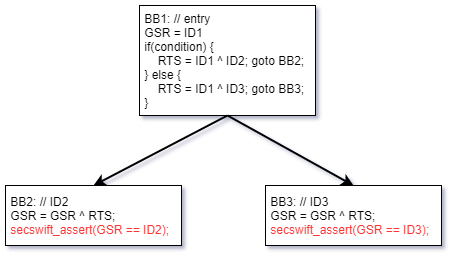
\includegraphics[width=0.55\textwidth]{ch6-ccpo/img/secswift-CF.png}
                \caption{Schéma de protection d'un branchement avec $SSCF$ \cite{Ferriere/LLVM19}}
                \label{fig:sscf-scheme}
                \end{figure}
            
                \textbf{Compteurs d'instructions}. La contre-mesure $CNT$ vise la protection contre le saut d'instruction niveau C en introduisant des compteurs incrémentés entre chaque instruction.
                Le listing \ref{lst:lalande} présente le début de la fonction \textit{verify\_pin} protégée avec $CNT$.
                Les macros \texttt{INCR} et \texttt{CHECK\_INCR} effectuent l'incrémentation d'un compteur, la seconde ajoutant un détecteur pour vérifier que celui-ci vaut bien la valeur attendue.
                Diverses macros sont proposées dans \cite{lalande} afin de protéger différentes structures (appel de fonction, boucle, condition...). La version étudiée ici est légèrement modifiée par rapport au papier original, certaines macros ajoutant un effet de bord dans la condition des détecteurs\footnote{Par exemple, la macro \texttt{CHECK\_INCR(cnt,val, det\_id) cnt = (cnt == val ? cnt + 1 : detect(det\_id));} dans sa version originale modifie le compteur dans le cas où une erreur est détectée. La vérification (détecteur) et la ré-initialisation du compteur ont donc été séparées.}.
             
\begin{minipage}{0.93\linewidth}
\lstset{escapeinside={<@}{@>}, label=lst:lalande}
\begin{lstlisting}
#define <@{\color{red!95} INCR}@>(cnt,val)  cnt = cnt + 1;
#define <@{\color{red!95} CHECK\_INCR}@>(cnt,val, cm_id) if(cnt != val) detect(cm_id); \
cnt = cnt + 1;
[...]


bool verify_pin(<@{\color{red!95}uint8\_t* CNT\_0\_VP\_1}@>) 
{
<@{\color{red!95} CHECK\_INCR(*CNT\_0\_VP\_1, CNT\_INIT\_VP + 0, 0LL)}@>
g_authenticated = 0;
<@{\color{red!95} CHECK\_INCR(*CNT\_0\_VP\_1, CNT\_INIT\_VP + 1, 1LL)}@>
<@{\color{red!95} DECL\_INIT(CNT\_0\_byteArrayCompare\_CALLNB\_1, CNT\_INIT\_BAC)}@>
<@{\color{red!95} CHECK\_INCR(*CNT\_0\_VP\_1, CNT\_INIT\_VP + 2, 2LL)}@>
bool res = byteArrayCompare(user_pin, card_pin, PIN_SIZE<@{\color{red!95}, \&CNT\_0\_compare\_CALLNB\_1}@>);
[...]
\end{lstlisting}
\end{minipage}

            \subsubsection{Détecteurs retirés}
            \label{sec:ch6:exp:results}
                
                La table \ref{tbl:ch6:exp:ccpo-all} présente les résultats obtenus pour les différents exemples.
                La colonne "Programme" indique quel programme de base est utilisé et la colonne "Contre-mesure" indique la contre-mesure systématique ajoutée ("-" indiquant qu'aucune contre-mesure n'est ajoutée). 
                La troisième colonne correspond au nombre global de détecteurs (après l'ajout de la contre-mesure).
                Les colonnes suivantes indiquent le pourcentage de détecteurs retirés après l'application de la méthodologie.
                         
                \begin{table}[htbp]
                \caption{Pourcentage de détecteurs retirés pour différents programmes}\label{tbl:ch6:exp:ccpo-all}
                \begin{center}
                \begin{tabular}{cc|c|ccc}
                    Programme & Contre-mesure & $\mathcal{D}(P)$ & 1 faute   & 2 fautes   & 3 fautes   \\
                    \hline
                    \hline
                    vp2c       & TD            & 11         & 72\% & 63\% & 18\% \\
                    vp2c       & SSCF          & 13         & 92\% & 76\% & 23\% \\
                    vp2c       & CNT           & 31         & 93\% & 93\% & 32\% \\
                    \hline
                    fu0       & TD            & 14         & 0\%  & 0\%  & 0\%  \\
                    fu0       & SSCF          & 24         & 12\% & 12\% & 8\%  \\
                    \hline
                    gc1       & -             & 11         & 81\% & 72\% & 63\% \\
                    gc1       & TD            & 39         & 37\% & 34\% & 34\% \\
                    gc1       & SSCF          & 38         & 57\% & 28\% & 28\% \\
                    \hline
                    aes rk    & TD            & 2          & 50\% & 50\% & 0\%  \\
                    aes rk    & SSCF          & 3          & 66\% & 33\% & 0\%  \\
                    \hline
                    aes c     & TD            & 8          & 50\% & 50\% & 0\%  \\
                    aes c     & SSCF          & 13         & 76\% & 61\% & 38\%
                    \end{tabular}
                \end{center}
                \end{table} 
                        
                On constate que le nombre de détecteurs retirés dépend fortement du programme et de la contre-mesure considérée. Naturellement, plus la limite de fautes est élevée, plus les détecteurs sont nécessaires.
                L'exemple $vp2c + CNT$ est un cas où la contre-mesure n'est pas prévue pour le modèle de faute considéré ($CNT$ visant la protection contre les sauts d'instruction au niveau C), ce qui explique pourquoi autant de détecteurs peuvent être retirés (jusqu'à 2 fautes).
                Dans certains exemples (tels que $fu0 + TD$ ou bien $aes$ $rk$ en 3 fautes), il n'est simplement pas possible de retirer de détecteurs.
                
            \subsubsection{Impact de l'objectif d'attaque}
            \label{sec:ch6:exp:phi}
        
                La table \ref{tbl:ch6:exp:vp-td-phi} présente les résultats obtenus sur l'exemple $vp2c$, en fonction de l'objectif d'attaque considéré: $\phi_{auth}$ (s'authentifier malgré un PIN incorrect), $\phi_{ptc}$ (ne pas décrémenter le compteur d'essais), leurs disjonction et conjonction logiques ($\phi_{auth\; \vee \;ptc}$ et $\phi_{auth\; \wedge \;ptc}$), ainsi que l'objectif d'attaque $\phi_{true}$ où toutes les traces sont considérées (hors cas d'erreurs).

                \begin{table}[htbp]
                \caption{Pourcentage de détecteurs retirés en fonction de l'objectif d'attaque ($vp+td$)}\label{tbl:ch6:exp:vp-td-phi}
                \begin{center}
                    \begin{tabular}{l|lll}
                    Objectif d'attaque      & 1 faute & 2 fautes & 3 fautes \\
                    \hline
                    \hline
                    $\phi_{auth}$           & 83\%    & 72\%     & 18\%     \\
                    $\phi_{ptc}$            & 72\%    & 63\%     & 9\%      \\
                    $\phi_{auth\; \vee \;ptc}$  & 83\%    & 72\%     & 18\%     \\
                    $\phi_{auth\; \wedge \;ptc}$ & 72\%    & 63\%     & 9\%      \\
                    $\phi_{true}$           & 18\%    & 9\%      & 9\%     
                    \end{tabular}
                \end{center}
                \end{table} 
                
                Comme attendu, plus l'objectif d'attaque est général, moins il est possible de retirer de détecteurs.
                L'objectif d'attaque $\phi_{true}$ ne permet le retrait que de 18\% des détecteurs en une faute, mais en trois fautes, les résultats sont équivalents à ceux de $\phi_{ptc}$ (et donc de $\phi_{auth\; \wedge \;ptc}$).
                Par ailleurs, on constate que $\phi_{auth}$ est contenu dans $\phi_{ptc}$ ($\phi_{auth}$ est équivalent à $\phi_{auth\; \vee \;ptc}$ et $\phi_{ptc}$ est équivalent à $\phi_{auth\; \wedge \;ptc}$).
  
            \subsubsection{Performances}
            \label{sec:ch6:exp:perf}
        
                La table \ref{tbl:ccpo-metrics} présente les métriques d'exécution et de performance des expérimentations précédentes.
                Les colonnes "Programme", "Contre-mesure" et "$\mathcal{D}(P)$" ont la même signification que pour la table \ref{tbl:ch6:exp:ccpo-all}. 
                La colonne "Chemins" montre le nombre de chemins complétés et la colonne "Traces" correspond au nombres de traces (dans $T_{cs}^{nb}(P, M)$).
                La colonne "Temps (DSE)" indique le temps d'exécution de KLEE pour la génération des traces. 
                La dernière colonne "Temps (Analyse)" indique le temps de l'analyse d'optimisation de détecteurs combinant les étapes de classification et de sélection.
        
                On peut constater que l'exploration des chemins est toujours le facteur limitant pour tous les programmes de test.
                La durée de l'analyse est fortement liée au nombre de traces, la classification en faisant un parcours complet.
                L'étape de sélection est négligeable dans tous les exemples traités, dû au faible nombre de traces contenant uniquement des détecteurs répétitifs, même pour les cas avec un nombre de traces élevé.

                \begin{table}[htbp]
                \centering
                {\small
                    \setlength\tabcolsep{3pt}
                    \begin{tabular}{ll|lll|ll}
                    Programme & Contre-mesure & $\mathcal{D}(P)$ & Chemins & Traces & Temps (DSE) & Temps (Analyse) \\
                    \hline
                    \hline
                    $vp$ & $TD$ & 11 & 7118 & 296 & \texttt{0:00:03} & 26ms \\
                    $vp$ & $SSCF$ & 13 & 130 576 & 1005 & \texttt{0:01:54} & 89ms \\
                    $vp$ & $CNT$ & 31 & 1 173 312 & 37 347 & \texttt{0:38:24} & 371ms \\
                    \hline
                    $fu$ & $TD$ & 14 & 935 409 & 43 328 & \texttt{0:39:16} & 736ms \\
                    $fu$ & $SSCF$ & 24 & 1 490 767 & 91 713 & \texttt{1:04:39} & 4s \\
                    \hline
                    $gc1$ & - & 11 & 4628 & 78 & \texttt{0:00:04} & 12ms \\
                    $gc1$ & $TD$ & 39 & 102 169 & 10 281 & \texttt{0:01:35} & 1s \\
                    $gc1$ & $SSCF$ & 38 & 1 048 354 & 58 367 & \texttt{0:31:45} & 2s \\
                    \hline
                    $aes rk$ & $TD$ & 2 & 9 439 & 847 & \texttt{0:00:07} & 61ms \\
                    $aes rk$ & $SSCF$ & 3 & 410 095 & 6 952 & \texttt{0:09:19} & 195ms \\
                    \hline
                    $aes$ & $TD$ & 8 & 1 064 007 & 38 810 & \texttt{1:17:25} & 575ms \\
                    $aes$ & $SSCF$ & 13 & 842 583 & 29 770 & \texttt{1:45:00} & 2s
                    \end{tabular}
                }
                \caption{Métriques de temps en 3 fautes \label{tbl:ccpo-metrics}}
                \end{table}
        
    \section{Conclusion, limitations et perspectives}
    \label{sec:ccpo-conclusion}
    
        Les sections précédentes ont décrit une méthodologie d'analyse de contre-mesures à détecteur permettant de retirer les tests sans introduire de nouvelles attaques.
        L'exécution avec détecteurs non bloquants permet d'effectuer une seule exploration des traces d'exécutions, ce qui rend l'analyse réaliste même pour des programmes contenant un nombre important de détecteurs. Les expérimentations effectuées montrent que les résultats sont très dépendants des programmes et des contre-mesures considérés mais qu'il reste possible de retirer des détecteurs dans la grande majorité des exemples étudiés.        
        La correction de cette approche est dépendante de celle de la méthode de génération des traces sous-jacente. L'implémentation dans Lazart avec l'exécution symbolique dépend donc de la complétude et de la correction des traces produites par KLEE.
        
        L'exécution avec détecteurs non bloquants impose certaines propriétés sur les détecteurs étudiés, ce qui rend l'analyse incomplète pour certaines contre-mesures (comme la contre-mesure $CNT$ \cite{lalande} qui a dû être modifiée en partie).        
        La protection des détecteurs est également un problème qui est difficile à résoudre. Seule la protection simple pour l'inversion de test a été implémentée, une sur-approximation de la nécessité d'un détecteur est possible lorsqu'une trace forçant le passage en contre-mesure est détectée.
        
        Retirer le corps de contre-mesure en plus des détecteurs n'est pas une question triviale.         
        Dans le cas général, c'est-à-dire un programme $P$ protégé contre n'importe quel type de contre-mesure à détecteurs, il est difficile de savoir quelles parties du corps des contre-mesures peuvent être retirées à partir de l'ensemble de détecteurs conservés (par exemple pour la contre-mesure \gls{SSCF}  où la variable $GSR$ dépend des identifiants précédents). 
        Des analyses statiques adaptées pour l'injection de fautes sont une piste d'exploration.
        
        La méthodologie présentée dans ce chapitre autorise qu'une attaque $a' \in T(P')$ corresponde à une attaque $a \in T(P)$ mais avec un nombre de fautes nécessaires plus petit en raison des détecteurs qui ont été retirés.
        Il est possible d'adapter la méthodologie en imposant que certaines attaques ne soient pas simplifiée de la sorte, en considérant comme nécessaire tout détecteur correspondant aux points d'injection de ces attaques. Associer le détecteur correspondant à une faute est simple dans le cas de contre-mesures à granularité de l'ordre du point d'injection, comme \gls{TM} ou \gls{SSCF} par exemple, mais ne l'est pas dans le cas général.  
        
        Par ailleurs, les expérimentations présentées dans ce chapitre ont été réalisées sur une ancienne version de l'outil, l'optimisation de contre-mesures n'ayant pas été mise-à-jour sur la version 4 actuelle (présentée dans le chapitre \ref{chpt:lazart} et \ref{chpt:lazart-implem}).
        La mise à jour sur la version actuelle permettrait de profiter du modèle de faute sur les données (\gls{DL}) et la combinaison de modèles.
        De la même manière cela permettrait d'étendre les expérimentations aux contre-mesures \gls{LM}.